% Created 2024-04-08 Mon 20:37
% Intended LaTeX compiler: pdflatex
\documentclass[a4paper, 11pt]{article}
\usepackage[utf8]{inputenc}
\usepackage[T1]{fontenc}
\usepackage{graphicx}
\usepackage{longtable}
\usepackage{wrapfig}
\usepackage{rotating}
\usepackage[normalem]{ulem}
\usepackage{amsmath}
\usepackage{amssymb}
\usepackage{capt-of}
\usepackage{hyperref}
\usepackage{lmodern} % Ensures we have the right font
\usepackage[T1]{fontenc}
\usepackage{inputenc}
\usepackage{graphicx, float}
\usepackage{amsmath, amsfonts, amsthm, amssymb, lipsum}
\usepackage[table, xcdraw]{xcolor}
\usepackage[colorlinks]{hyperref}
\hypersetup{colorlinks, linkcolor=blue, urlcolor=blue}
\setlength{\parindent}{0pt}
\setlength{\parskip}{1em}
\usepackage[stretch=10]{microtype}
\usepackage{hyphenat}
\usepackage{ragged2e}
\usepackage{subfig} % Subfigures (not needed in Org I think)
\usepackage{hyperref} % Links
\usepackage{listings} % Code highlighting
\usepackage[margin=1in, footskip=0.25in]{geometry}
\renewcommand{\baselinestretch}{1.15}
\pagenumbering{gobble}
\usepackage[explicit]{titlesec}
\usepackage{enumitem}
\setlist[itemize]{topsep=0pt}
\newtheorem{theorem}{Theorem}[section]
\newtheorem{corollary}{Corollary}[theorem]
\newtheorem{lemma}[theorem]{Lemma}
\newtheorem{definition}{Definition}[theorem]
\setlength{\abovedisplayskip}{-15pt}
\setlength{\belowdisplayskip}{0pt}
\setlength{\abovedisplayshortskip}{0pt}
\setlength{\belowdisplayshortskip}{0pt}
\author{Bryan Lim Jing Xiang (A0233605M)}
\date{}
\title{Task A1}
\hypersetup{
 pdfauthor={Bryan Lim Jing Xiang (A0233605M)},
 pdftitle={Task A1},
 pdfkeywords={},
 pdfsubject={},
 pdfcreator={Emacs 29.3 (Org mode 9.7)}, 
 pdflang={English}}
\begin{document}

\maketitle
\section{Dataset}
\label{sec:orga4dd47c}
\subsection{Overview}
\label{sec:org951bf28}
This dataset consists of a list of animes scrapped from anime recommendation systems such as Anime Planet. The data that is of interest includes the following:

\begin{center}
\begin{tabular}{lll}
Field & Description & Data Type\\[0pt]
\hline
Rank & Rank of the anime based on rating & Integer (Starting from 1)\\[0pt]
Name & Anime Name & String\\[0pt]
Studio & The studio that produced the anime & String\\[0pt]
Release Season & Season in which the anime was released & ['Spring', 'Summer', 'Autumn', 'Winer']\\[0pt]
Release Year & Year in which the anime was released & Year as integer\\[0pt]
Tags & List of all the genres/tags the anime belong to & Space-delimited string\\[0pt]
Ratings & Rating of the anime & Integer - Rating is out of 5\\[0pt]
 &  & \\[0pt]
\end{tabular}
\end{center}

This dataset is interesting in that it allows us to analyse the popularity and trends in the anime industry across many different years and seasons.
\subsection{Data origin}
\label{sec:org383e295}
\url{https://www.kaggle.com/datasets/vishalmane10/anime-dataset-2022}
\subsection{Github Repository}
\label{sec:org66211e4}
\url{https://github.com/bryanljx/visualisation}
\section{Purpose of Visualisation}
\label{sec:org83f4fc5}
For this dataset, the query of interest is: ``What are the trends amongst popular animes across the years? As a follow up, what constitutes the success or popularity of an anime?''

Such a query is naturally of interest to stakeholders such as:
\begin{itemize}
\item Anime Watchers
\begin{itemize}
\item Get recommendations on what types of animes to watch from the trending genres as well as anime studios that produce the best animes
\end{itemize}
\item Potential Investors
\begin{itemize}
\item Learn about genres that are popular as well as which studios have always been producing the best animes
\end{itemize}
\end{itemize}
\section{Visualisation}
\label{sec:orgf6a8234}
\subsection{Breakdown of genres of top 100 animes of all time}
\label{sec:orgd186c51}

\begin{center}
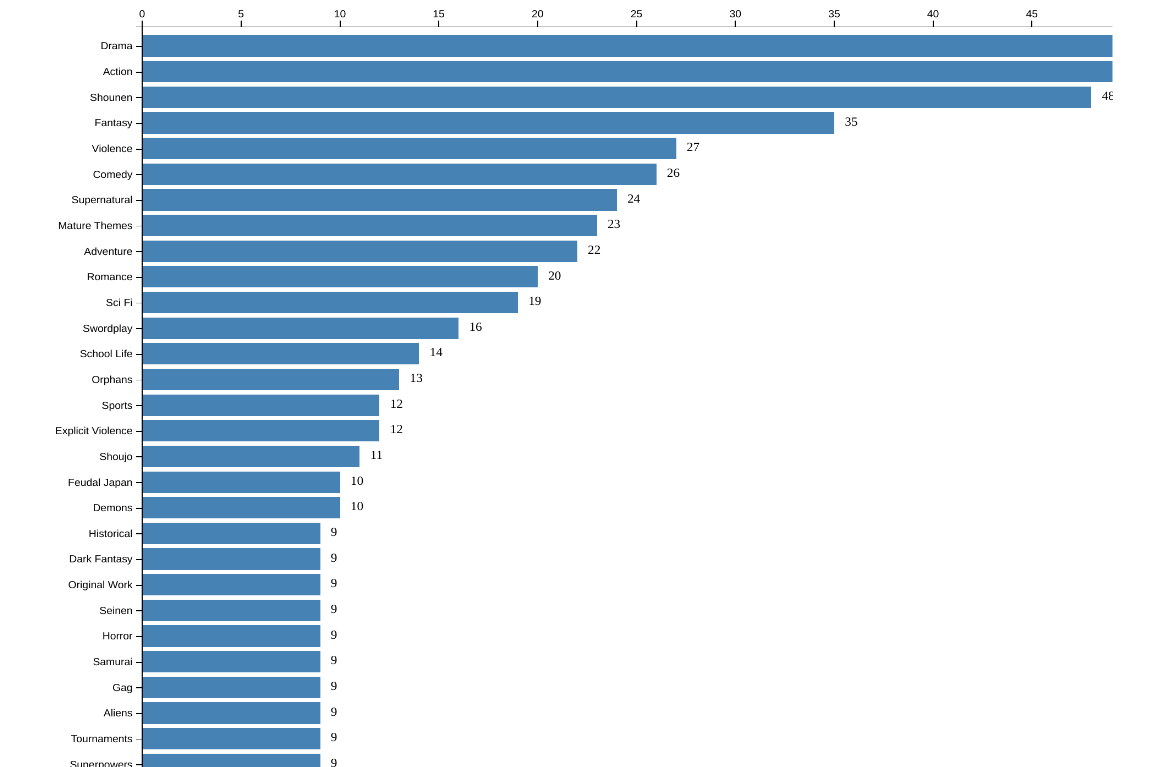
\includegraphics[width=.9\linewidth]{./charts/anime_genre_across_time.png}
\end{center}

\begin{itemize}
\item A horizontal bar chart was chosen here to show the number of top 100 animes of all time that falls into the various genres.
\begin{itemize}
\item Note: The image was cut off slightly when saving to pdf/screenshot, please load and view the actual webpage instead.
\end{itemize}
\item Visual encoding here includes:
\begin{itemize}
\item Length - Denoting the number of animes that belong to that genre
\end{itemize}
\end{itemize}
\subsection{Breakdown of anime studios behind top 100 animes of all time}
\label{sec:org705235f}

A\begin{center}
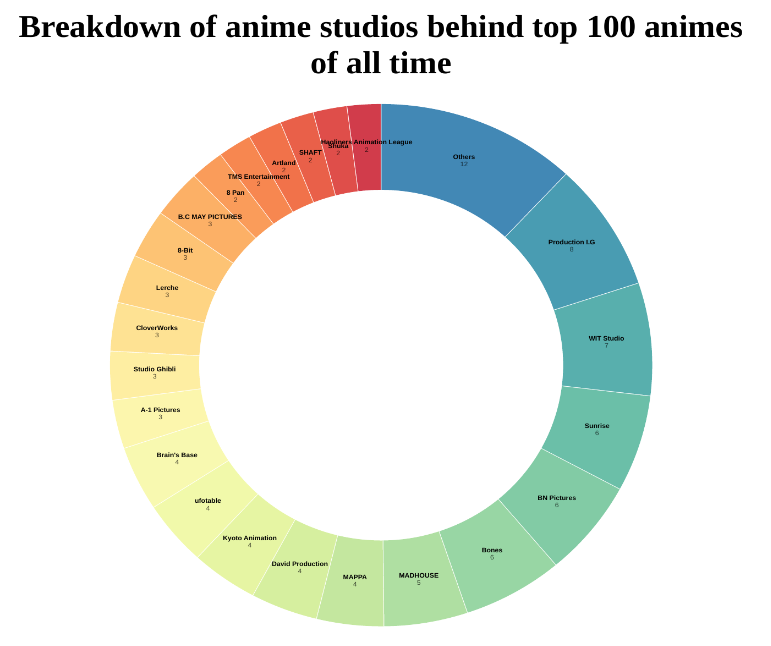
\includegraphics[width=.9\linewidth]{./charts/anime_studios.png}
\end{center}

\begin{itemize}
\item A pie chart was chosen to show the distribution/percentages of the anime studios that have produced the most number of top 100 animes of all time.
\item Visual encoding here includes:
\begin{itemize}
\item Length - Denoting the number of such animes produced
\item Color - Differentiating the anime studios
\end{itemize}
\end{itemize}
\subsection{Number of anime per genre (for the top 10 genres all time) across the year 2000 - 2022}
\label{sec:orgd6b66c3}
\begin{center}
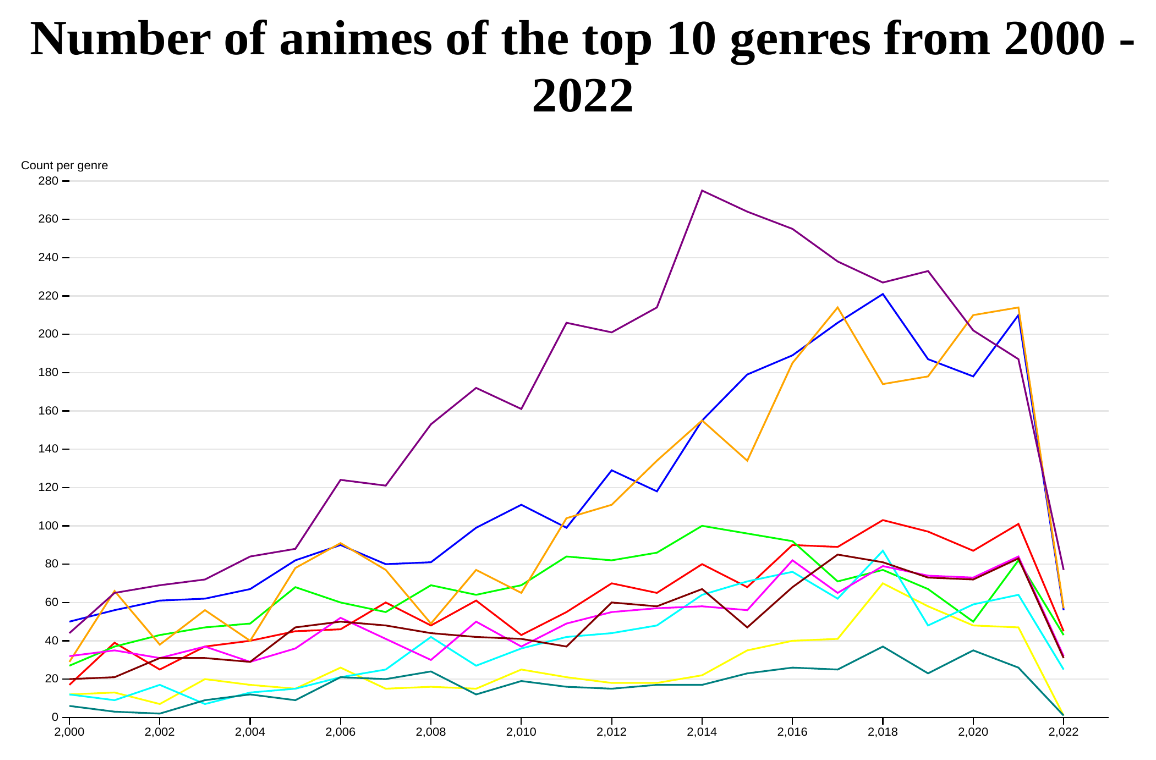
\includegraphics[width=.9\linewidth]{./charts/anime_per_genre.png}
\end{center}
\begin{itemize}
\item A line chart was chosen here to display and compare the patterns in the number of animes produced across the years for the top 10 best performing genres of all time.
\item Visual encoding here includes:
\begin{itemize}
\item Position - Denoting the magnitude/count of animes per genre
\item Color - Differentiating the different genre
\end{itemize}
\end{itemize}
\end{document}
